\subsection{The Feature Traceability Problem}
\begin{frame}{\myframetitle}
	\begin{mycolumns}
		\todots
	\mynextcolumn
		\todots
	\end{mycolumns}
\end{frame}

\subsection{Feature Location}
\begin{frame}{\myframetitle}
	\begin{mycolumns}
		\todots
	\mynextcolumn
		\todots
	\end{mycolumns}
\end{frame}

\subsection{Feature Traceability with Colors}
\begin{frame}{\myframetitle}
	\begin{mycolumns}
		\myexampletight{Tool Support for Feature Traceability}{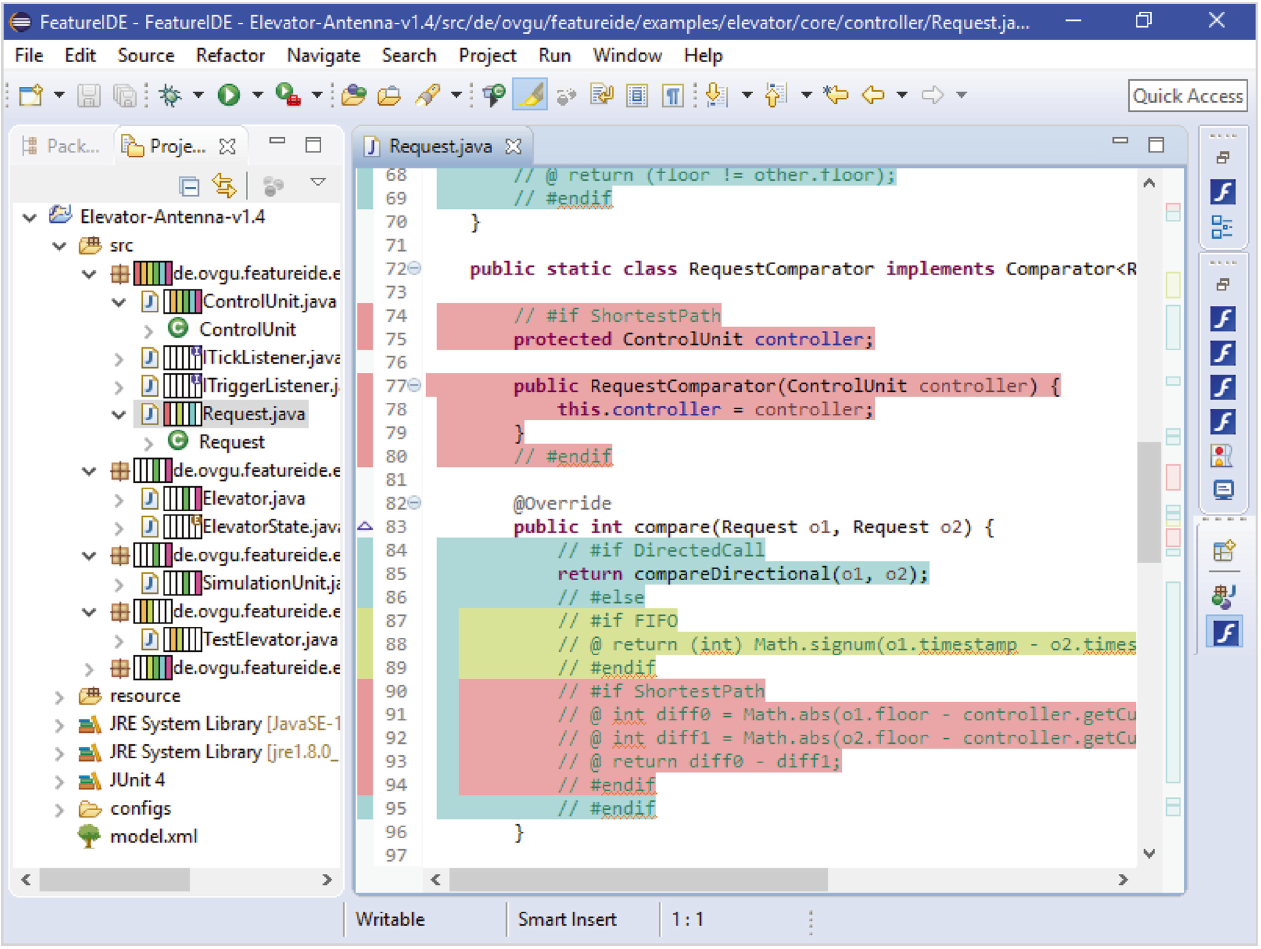
\includegraphics[width=\linewidth]{feature-traceability}}
	\mynextcolumn
		\todots
	\end{mycolumns}
\end{frame}
% FeatureCommander

\subsection{Recap: Scattering, Tangling, Replication}
\begin{frame}{\myframetitle}
	\begin{mycolumns}
		\todots
	\mynextcolumn
		\todots
	\end{mycolumns}
\end{frame}

\subsection{Virtual Separation of Concerns}
\begin{frame}{\myframetitle}
	\begin{mycolumns}
		\todots
	\mynextcolumn
		\todots
	\end{mycolumns}
\end{frame}
% no preprocessor directives
% CIDE
% forward reference to physical separation of concerns in next two lectures
